\documentclass[a4paper]{article}
\usepackage[utf8]{inputenc}
\usepackage{fancyhdr}
\usepackage{vmargin}
\usepackage{listings}

%nicer tables
\usepackage{booktabs}

\usepackage{graphicx}

\usepackage{float}

\usepackage{color}
\usepackage{url}
\usepackage{hyperref}

\usepackage{enumerate}

\usepackage[backend=biber]{biblatex}

\usepackage{multicol}
\setlength{\columnsep}{1cm}
\setlength{\headheight}{36pt}

\definecolor{bluekeywords}{rgb}{0.13,0.13,1}
\definecolor{greencomments}{rgb}{0,0.5,0}
\definecolor{redstrings}{rgb}{0.9,0,0}



%
\usepackage{amsmath, amsthm, amssymb}
\usepackage[ngerman, english]{babel}
\usepackage{marvosym}
\usepackage{graphics}
\usepackage{extarrows}
\usepackage{forloop}
\usepackage{mathtools}

\usepackage[]{algorithm2e}

\usepackage{hyperref}% http://ctan.org/pkg/hyperref
\usepackage{cleveref}% http://ctan.org/pkg/cleveref
\usepackage{lipsum}% http://ctan.org/pkg/lipsum
\newtheorem{definition}{Definition}
\newtheorem{theorem}{Theorem}
\newtheorem{lemma}{Lemma}
\newtheorem{preliminary}{Preliminary}
\newtheorem{notation}{Notation}
\newtheorem{property}{Property}
\newtheorem{corollary}{Corollary}
\newtheorem{example}{Example}
\newtheorem{hypothesis}{Hypothesis}

\crefname{theorem}{Theorem}{Theorems}
\crefname{definition}{Definition}{Definitions}
\crefname{lemma}{Lemma}{Lemmas}
\crefname{preliminary}{Preliminary}{Preliminaries}
\crefname{notation}{Notation}{Notations}
\crefname{property}{Property}{Properties}
\crefname{corollary}{Corollary}{Corollaries}
\crefname{example}{Example}{Examples}
\crefname{hypothesis}{Hypothesis}{Hypotheses}

\newenvironment{beweis}{\begin{proof}[Beweis]}{\end{proof}}
%



\lstset{language=Python,
showspaces=false,
showtabs=false,
breaklines=true,
showstringspaces=false,
breakatwhitespace=true,
escapeinside={(*@}{@*)},
commentstyle=\color{greencomments},
keywordstyle=\color{bluekeywords}\bfseries,
stringstyle=\color{redstrings},
basicstyle=\ttfamily
}


\setlength{\parindent}{0pt}
\setlength{\parskip}{5pt}

\frenchspacing
\pagestyle{fancy}
\sloppy 

\markright{headline}

\addbibresource{references.bib}

\begin{document}

\lhead{\begin{tabular}{l}
\\
Neural Networks\\
Saarland University WiSe 2020/2021\\
\end{tabular}}

\rhead{\begin{tabular}{r}
Assignment 5\\
Simon Laurent Lebailly, 2549365\\%% <=== Also HERE if you have a team mateUpdate Name HERE !!! 
Christian Schmidt, 2537621
\end{tabular}}




\section*{Exercise 5.1 - Gradient Descent}
$(1+0,5+1 = 2,5 \text{ points})$
    \subsection*{a)}
        
        
        
    \subsection*{b)}
        
        
        
    \subsection*{c)}
        
    
    
        


\newpage
\section*{Exercise 5.2 - Weight Space Symmetry}
$(1+0,5 = 1,5 \text{ points})$
    \subsection*{a)}
        
    
    
    \subsection*{b)}
        



\newpage
\section*{Exercise 5.3 - Hessian and Optimization}
$(1+1 = 2 \text{ points})$
    \subsection*{\underline{Figure (a):}}
        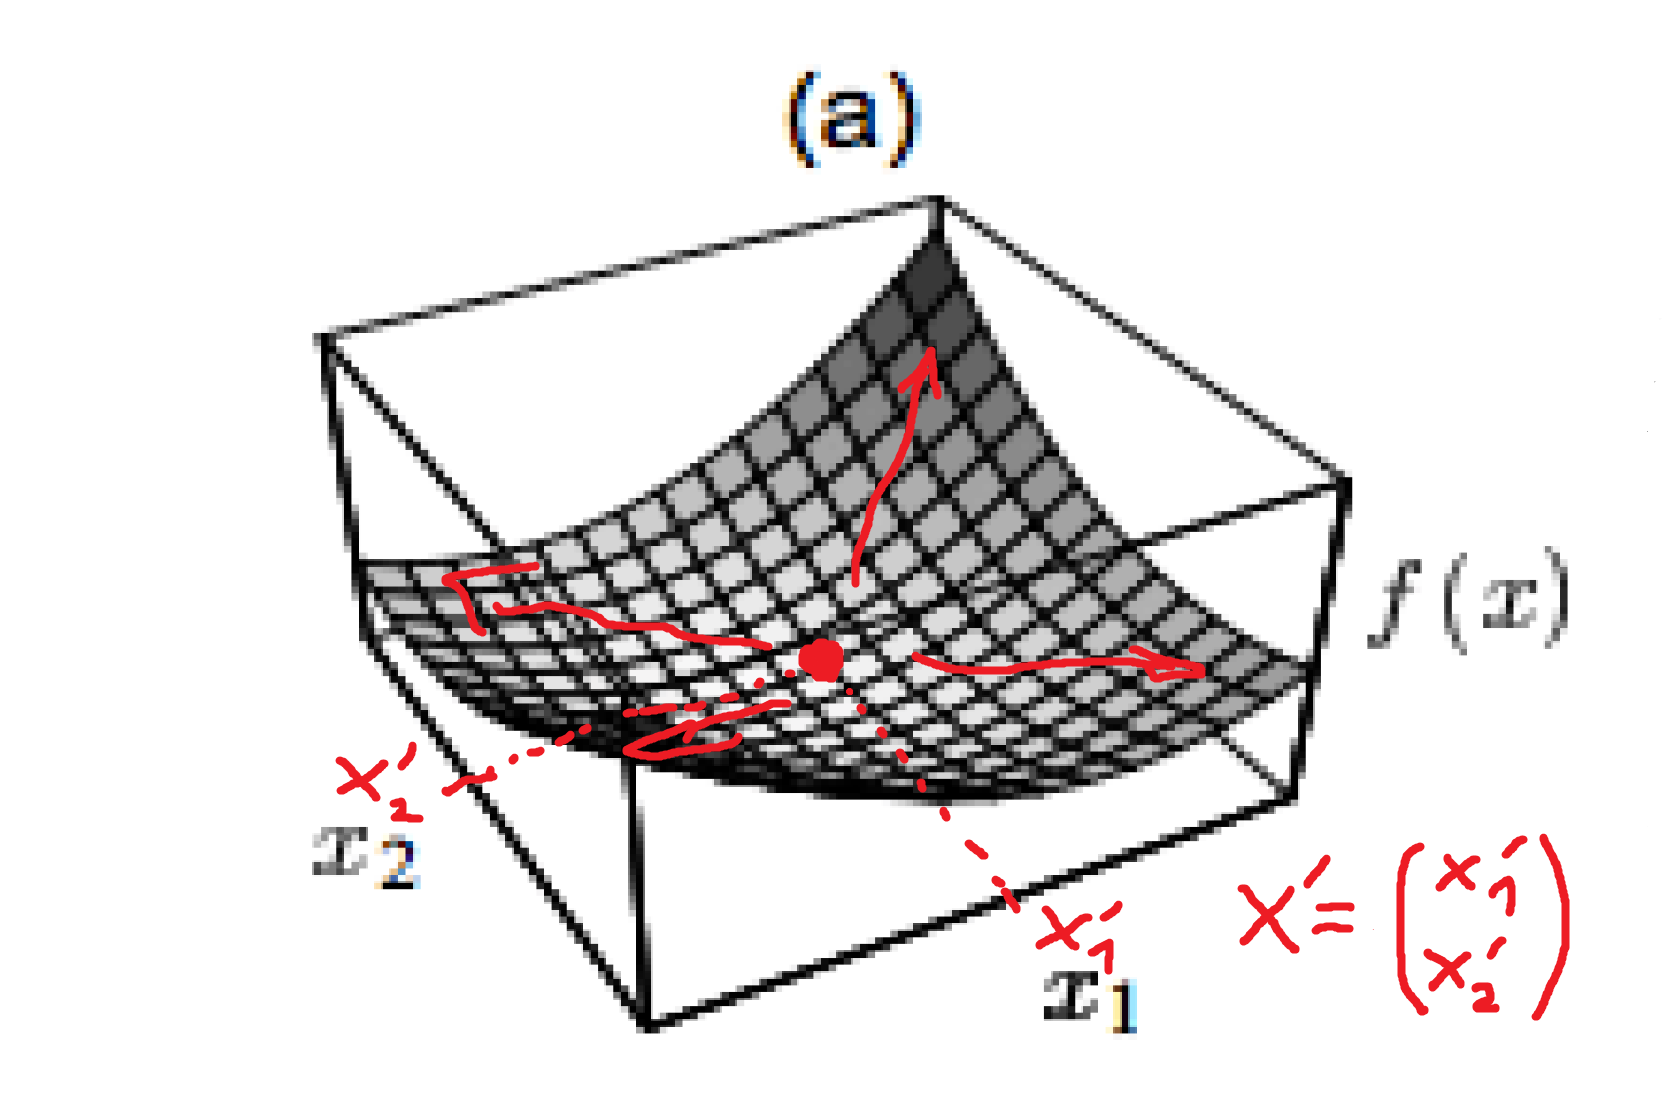
\includegraphics[width=0.8\linewidth]{Assignment 5/1.png}
        \subsubsection*{a)}
            At any given point, the eigenvalues of the Hessian matrix tell us whether the surface is concave up, concave down, or a little of both.
            As we can see, $x'$ is a local extremum of $f(x)$. To be more precise, $x'$ seems to be a local minimum.
            And from the view of the representative red arrows, the function $f(x)$ is increasing from $x'$ in all directions.
            Hence the surface of the function is concave up from the view of point $x'$.
            As a function that maps from two dimensional space, the Hessian matrix has exactly two eigenvectors, and therefore exactly two eigenvalues.
            Looking at the slope, the function is increasing in all directions from $x'$ as just mentioned.
            As we know from the exercise description, the curvature in the direction of an eigenvector is determined by its eigenvalue.
            Thus, all eigenvalues have a positive sign.

        \subsubsection*{b)}
            Since all eigenvalues of the symmetric Hessian matrix $A$ are greater than zero, we can conclude that $X^T A X$ is greater than zero, and thus $A$ is positive definite per definition.


\newpage
    \subsection*{\underline{Figure (b):}}
        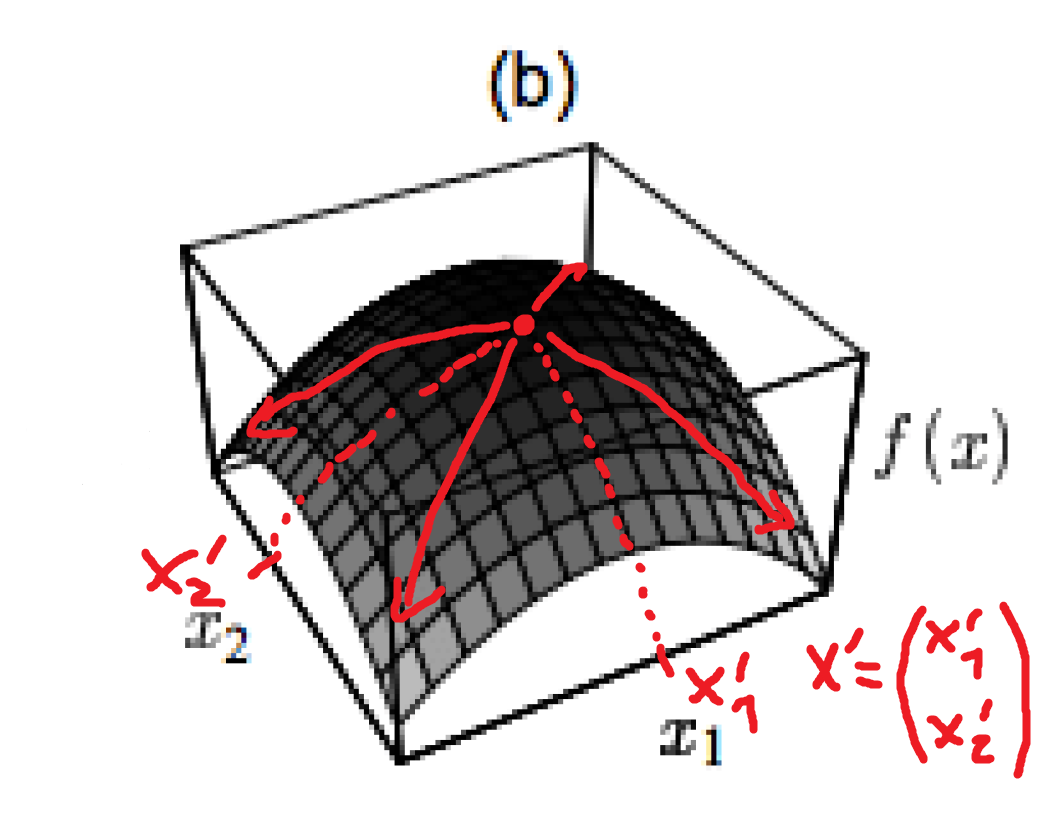
\includegraphics[width=0.8\linewidth]{Assignment 5/2.png}
        \subsubsection*{a)}
            At any given point, the eigenvalues of the Hessian matrix tell us whether the surface is concave up, concave down, or a little of both.
            As we can see, $x'$ is a local extremum of $f(x)$. To be more precise, $x'$ seems to be a local maximum.
            And from the view of the representative red arrows, the function $f(x)$ is decreasing from $x'$ in all directions.
            Hence the surface of the function is concave down from the view of point $x'$.
            As a function that maps from two dimensional space, the Hessian matrix has exactly two eigenvectors, and therefore exactly two eigenvalues.
            Looking at the slope, the function is decreasing in all directions from $x'$ as just mentioned.
            As we know from the exercise description, the curvature in the direction of an eigenvector is determined by its eigenvalue.
            Thus, all eigenvalues have a negative sign.

        \subsubsection*{b)}
            Since all eigenvalues of the symmetric Hessian matrix $A$ are less than zero, we can conclude that $X^T A X$ is less than zero, and thus $A$ is negative definite per definition.


\newpage
    \subsection*{\underline{Figure (c):}}
        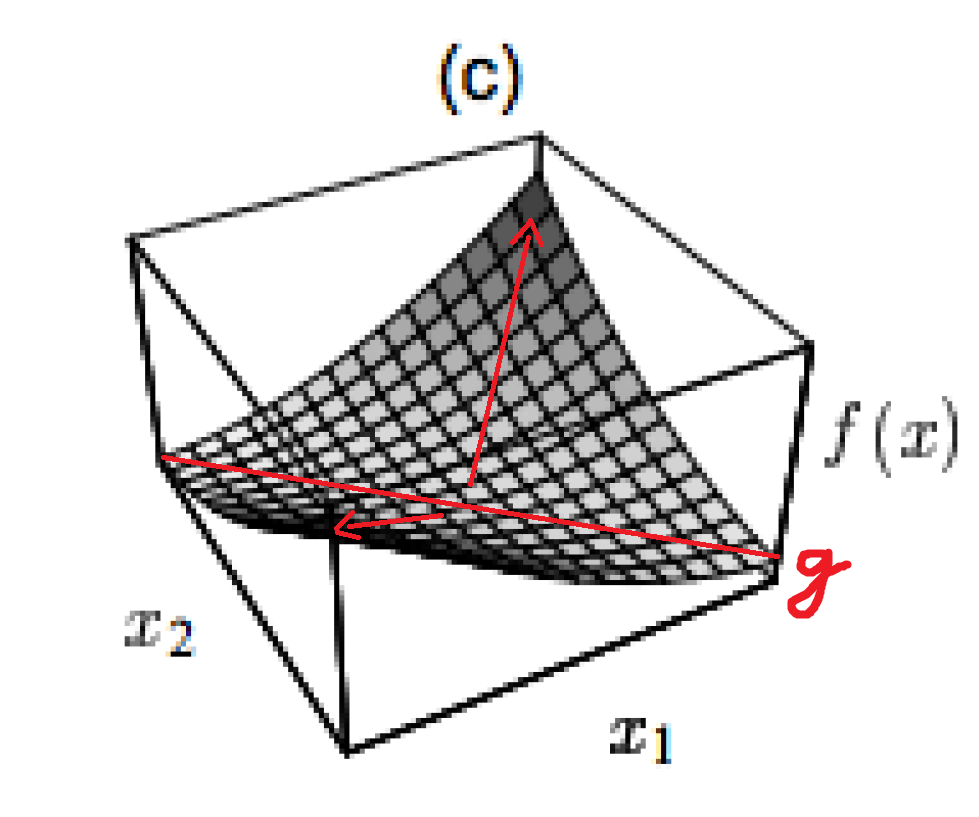
\includegraphics[width=0.8\linewidth]{Assignment 5/3.png}
        \subsubsection*{a)}
            $g$ represents a line, which has either a low or no gradient, and on this figure raises the question of a local minimum.
            Intuitively, we would assume from the problem that $g$ has no gradient. 
            But since we have to make this decision on the basis of a plot with poor resolution, we treat both cases for completeness!
            If $g$ has no gradient, there are an infinite number of extreme points (minimums), which all lie on the straight line $g$, and if $g$ has no gradient, there is not a single minimum.
            In both cases, however, there is no curvature in the direction of the straight line $g$.
            Only in the direction of the red arrows, i.e. orthogonal to $g$ in both directions, the surface is curved upwards.
            As a function that maps from two dimensional space, the Hessian matrix has exactly two eigenvectors, and therefore exactly two eigenvalues.
            Looking at the slope, the function only increases in the directions which are orthogonal to the direction of $g$.
            As we know from the exercise description, the curvature in the direction of an eigenvector is determined by its eigenvalue.\\
            Thus, one eigenvalue has a positive sign, the other is zero.

        \subsubsection*{b)}
            Since all eigenvalues of the symmetric Hessian matrix $A$ are greater or equal than zero, we can conclude that $X^T A X$ is greater or equal than zero, and thus $A$ is positive semidefinite per definition.
            But as required in the task, we have to decide if $A$ is positive definite, negative definite or neither.
            And since $A$ can not be positive or negative definite, the Hessian matrix is indefinite.


\newpage
    \subsection*{\underline{Figure (d):}}
        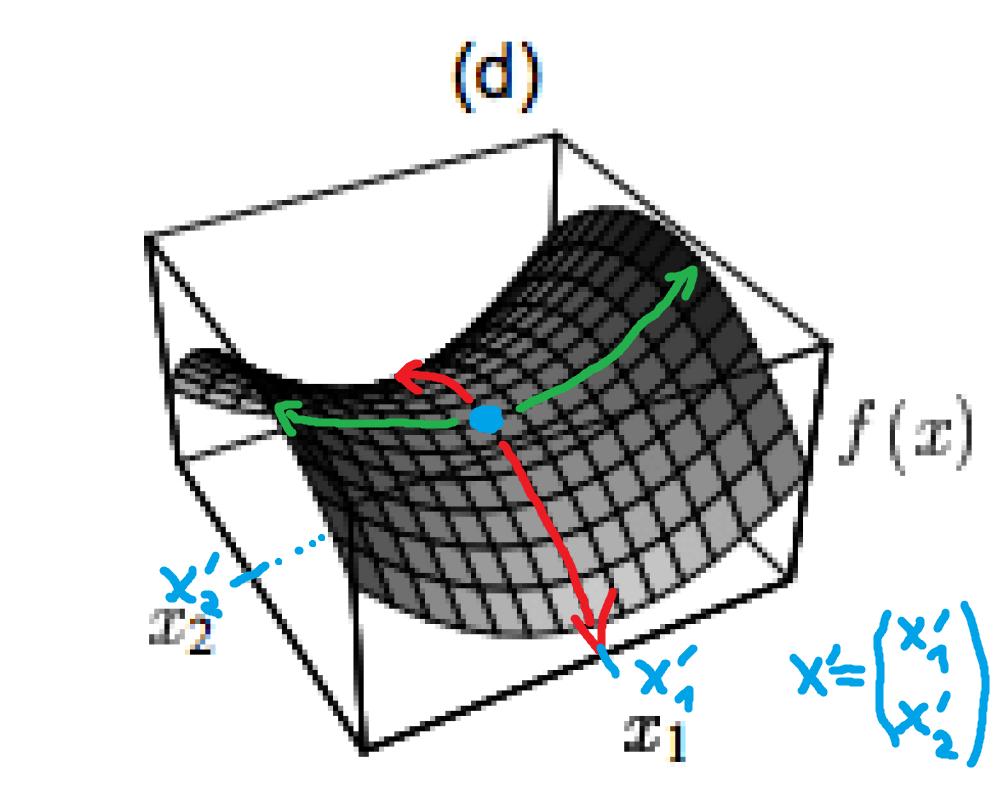
\includegraphics[width=0.8\linewidth]{Assignment 5/4.png}
        \subsubsection*{a)}
        
        \subsubsection*{b)}
            
            




\newpage
\section*{Exercise 5.4 - Gradient Descent and Newton's Method}
$(1+1+0,5 = 2,5 \text{ points})$
    \subsection*{a)}
        
        
        
    \subsection*{b)}
        
        
        
    \subsection*{c)}
    
    



\newpage
\section*{Exercise 5.5 - Convex Optimization}
$(0,5+0,5+0,5 = 1,5 \text{ points})$
    \subsection*{a)}
        
        
        
    \subsection*{b)}
        
        
        
    \subsection*{c)}
        
    
    





\end{document}
